\subsection{ソフトウェア構築の基礎}

ソフトウェア構築の基礎は、五つの考え方で整理できる。第一に複雑さを最小化すること、第二に変化を予期し受け入れること、第三に検証しやすく作ること、第四に資産を再利用すること、第五に標準を適用することである。これらは設計にも当てはまるが、構築では特にコード、テスト、部品、ツールに直接表れる。

\par\smallskip
\begin{center}
\centering
\IfFileExists{assets/generated_figures/ch04/fig-ch04-03.png}{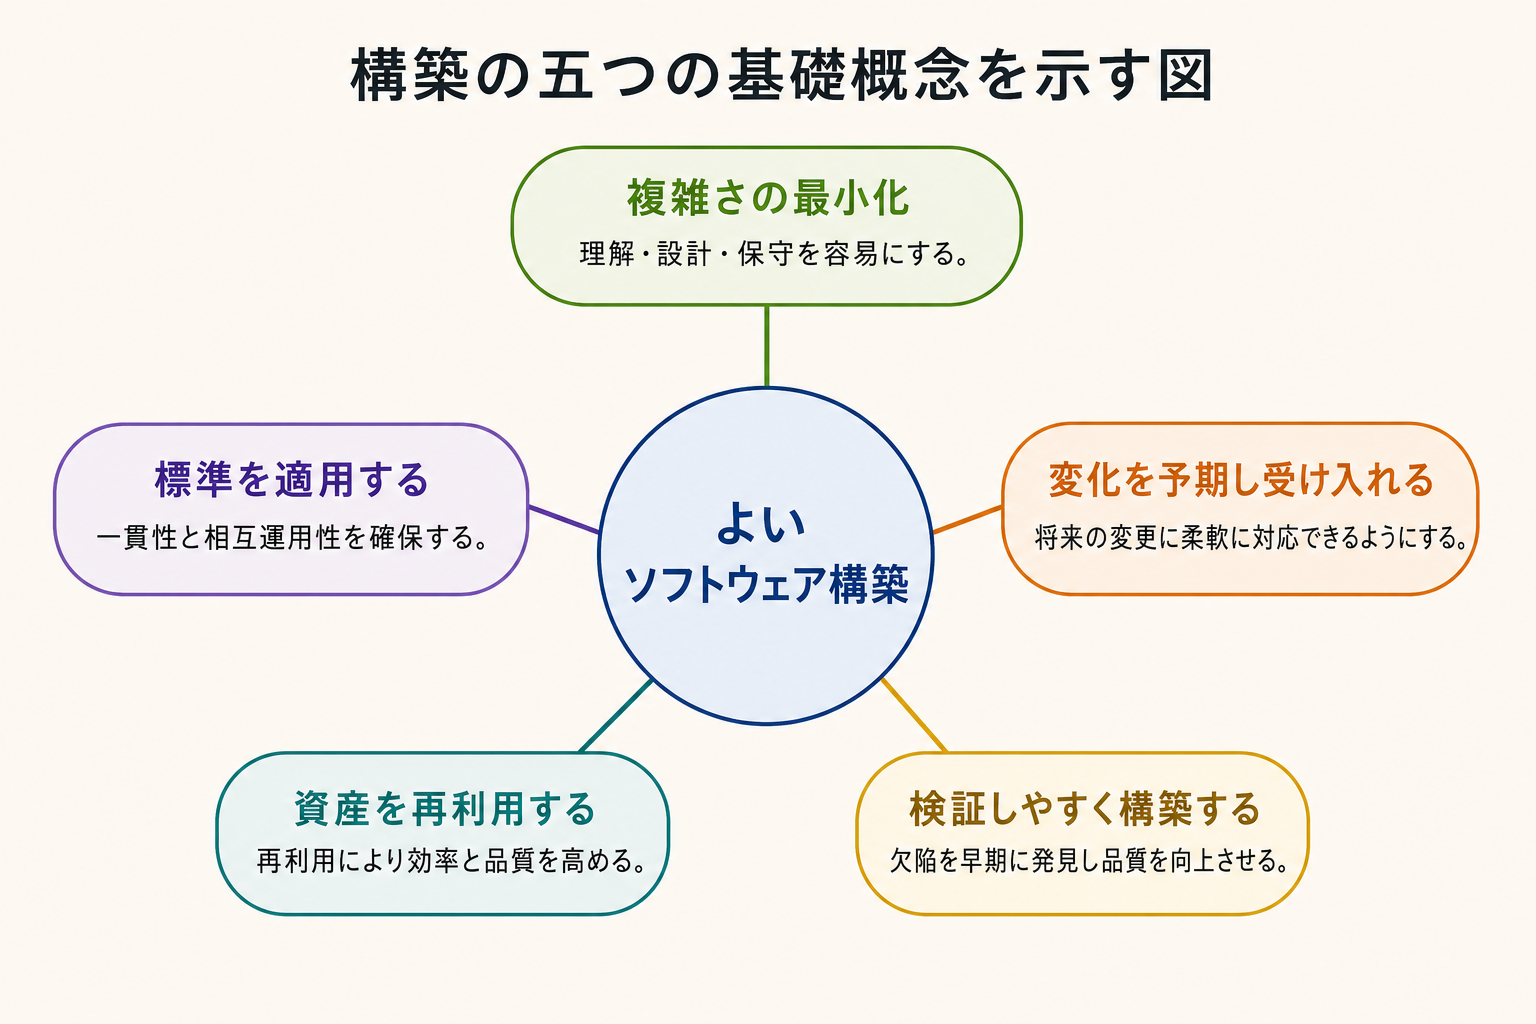
\includegraphics[width=0.96\linewidth]{assets/generated_figures/ch04/fig-ch04-03.png}}{\fbox{\parbox[c][48mm][c]{0.9\linewidth}{\centering 画像生成待ち\\構築の五つの基礎概念を示す図}}}
\par\smallskip
\refstepcounter{figure}\label{fig:ch04-03}図 \thefigure: 構築の五つの基礎概念を示す図
\end{center}
図 \thefigure は、構築の五つの基礎概念を示す図を視覚的に整理したものである。
\par\smallskip

\subsubsection{複雑さの最小化}

人間の作業記憶には限界がある。複雑な構造や大量の詳細を長時間正確に保持することは難しい。この限界は、ソフトウェア構築の中心課題である。コードが複雑になると、理解しにくく、テストしにくく、変更しにくくなる。したがって、構築では「賢そうなコード」よりも「単純で読みやすいコード」を優先する必要がある。

複雑さには複数の種類がある。条件分岐やループが多いコードは、実行経路が多くなる。依存関係が多いコードは、変更の影響範囲が広くなる。名前がわかりにくいコードは、読者の理解を妨げる。ビルド手順が複雑であれば、構築そのものが不安定になる。

循環的複雑度は、コードの制御フローの複雑さを測る代表的な指標である。大まかには、独立した実行経路の数を表す。値が大きいほど、理解やテストが難しくなる傾向がある。ただし、指標は判断の補助であり、指標だけでよいコードかどうかを決めてはならない。

複雑さを下げる実務上の手段には、命名規則、適切な関数分割、モジュール化、重複の排除、標準的な制御構造の利用、読みやすいレイアウト、レビュー、静的解析、単体テストがある。

\begin{keybox}{見分け方}
複雑なコードは、説明に時間がかかる。単純なコードは、名前、構造、流れから意図が読み取れる。構築では「動くか」だけでなく「次の人が読めるか」を基準にする必要がある。
\end{keybox}

\subsubsection{変化を予期し受け入れる}

多くのソフトウェアは時間とともに変わる。要求が変わることもあれば、利用者数、実行環境、ライブラリ、法規制、ビジネス方針が変わることもある。構築で変化を予期するとは、将来の変更が入ったときに、局所的な修正で済むように作ることである。

変化を予期するためには、拡張しやすい構造、明確なインタフェース、設定による切り替え、再利用可能な部品、テストによる安全網が必要である。一方で、まだ必要でない過剰な柔軟性を作り込むと、逆に複雑さが増える。したがって、予期すべき変化を見極め、過剰設計を避けることが重要である。

現代の開発では、変化を避けるのではなく受け入れる実践が広く使われる。アジャイル開発、DevOps、継続的デリバリ、継続的デプロイは、短い周期で変更を入れ、テストし、提供し、運用から学ぶための仕組みである。

\subsubsection{検証しやすく構築する}

検証しやすく構築するとは、コードを書いた人、テスト担当者、利用者が欠陥を見つけやすいようにソフトウェアを作ることである。これは、後でテストを追加すればよいという意味ではない。構築中から、テスト可能性を意識した設計と実装が必要である。

具体的には、単体テストを書きやすい関数分割、依存関係を差し替えやすい構造、複雑な言語機能の制限、ログによる挙動記録、コーディング標準、コードレビュー、入力値の検査、異常系の明示が役立つ。

検証しやすいコードでは、失敗が早く発見される。失敗が早く見つかるほど、原因に近い場所で修正できるため、修正費用を下げやすい。

\subsubsection{資産の再利用}

再利用とは、既存の資産を別の問題解決に使うことである。構築で再利用される資産には、フレームワーク、ライブラリ、モジュール、コンポーネント、ソースコード、商用既製品、クラウドサービスなどがある。

再利用には二つの側面がある。第一は、再利用されることを意識して作る「再利用のための構築」である。第二は、既存の資産を使って新しい解決策を作る「再利用による構築」である。前者では、汎用性、可変性、文書化、テストが重要になる。後者では、選定、評価、統合、ライセンス、保守、脆弱性管理が重要になる。

\begin{keybox}{注意}
再利用は必ず得とは限らない。再利用した部品に脆弱性、ライセンス問題、保守停止、過剰な依存があれば、後から大きな費用が発生する。再利用するものは、品質と責任範囲を確認する必要がある。
\end{keybox}

\subsubsection{構築における標準の適用}

\term{標準}{Standard}は、構築を効率化し、品質を安定させ、複数人の作業をそろえるために使う。標準には外部標準と内部標準がある。外部標準は、業界団体、国際標準化機関、プラットフォーム提供者などが定める。内部標準は、組織やプロジェクトが定める。

\term{構築}{Construction}に直接関係する標準には、文書形式、プログラミング言語、コーディング規約、例外処理方針、プラットフォームのインタフェース、ツール記法、UML などの表記法がある。特にセキュリティの観点では、許可する言語機能やライブラリ、禁止する危険な書き方を明確にすることが重要である。
